\chapter{Appendix}
\section{Discussions on Other Aggregate Functions in Chapter 4}
\label{sec:discussion}
First, we shall see that supporting \emph{sum} is equivalent
to supporting \emph{avg}. 
A ranked-streak which has a rank under \emph{avg} will have the 
same rank under \emph{sum} as the ranking is derived by comparing all 
candidates with the same length. 
%
Second, supporting \emph{count} is equivalent to supporting \emph{sum}. 
By assigning each event with a value of either 1 or 0, we can apply the 
same pruning bounds for \emph{sum} to support \emph{count}. 
%
Third, supporting \emph{max} is equivalent to supporting \emph{min}. This is 
because when \emph{max} is used as the aggregate function, we are more interested 
to find streaks which have smaller aggregation values. 
For example, ``XXX stock has a maximum of \$0.2 price
in consecutive 10 days, which is the lowest ever''. Then finding the sketches according to \emph{max} 
can be derived from \emph{min} directly by negating the event values. 
Therefore, we only provide bounds for 
\emph{sum} and \emph{min}, which are shown as in Table~\ref{tbl:agg_bound}.
%
%{\renewcommand{\arraystretch}{1.2} 
\begin{table}[h]
\caption{Bounds for other aggregate functions}
\centering
\begin{tabular}{|c|c|}
\hline 
\textbf{Aggregate Function} & \textbf{Subadditivity} \\
\hline 
\emph{sum} & $J_s(w) \leq J_s(w_1) + J_s(w-w_1) $ \\
\emph{min} & $J_s(w) \leq max(J_s(w_1), J_s(w-w_1))$ \\
\hline 
\textbf{Aggregate Function} & \textbf{Visting-Streak Bound} \\
\hline 
\emph{sum} & $J_s(w) = J_s(w-1)+J_s(1)$ \\
\emph{min} & $J_s(w) = J_s(w/2)$ \\
\hline 
\textbf{Aggregate Function}& \textbf{Unseen-Streak Bound} \\
\hline 
\emph{sum} & $M_s(w) = W_s(t,w).\overline{v} + J_s(t-w)$ \\
\emph{min} & $M_s(w) = max\{W_s(t,w).\overline{v}, J(1)\}$ \\
\hline 
\textbf{Aggregate Function }& \textbf{Online-Streak Bound} \\
\hline 
\emph{sum} & $M_s(w) = W_s(t,w).\overline{v} + J_s(t-w)$ \\
\emph{min} & $M_s(w) = max\{W_s(t,w).\overline{v}, J(1)\}$ \\
\hline 
\end{tabular} 
\label{tbl:agg_bound}
\end{table}
%}

We present the performance variations of our $k$-Sketch query under different aggregate functions in Fig.~\ref{exp:agg_cmp}. We can see from the figures that when adopting \emph{min} (\emph{max}) the performance in both online and offline scenarios drops (20\% to 30\%). This indicates that the pruning bounds in \emph{min} (\emph{max}) is weaker than \emph{avg} (\emph{sum}, \emph{count}).

\begin{figure}[h]
\centering
    \begin{subfigure}[b]{0.45\textwidth}
        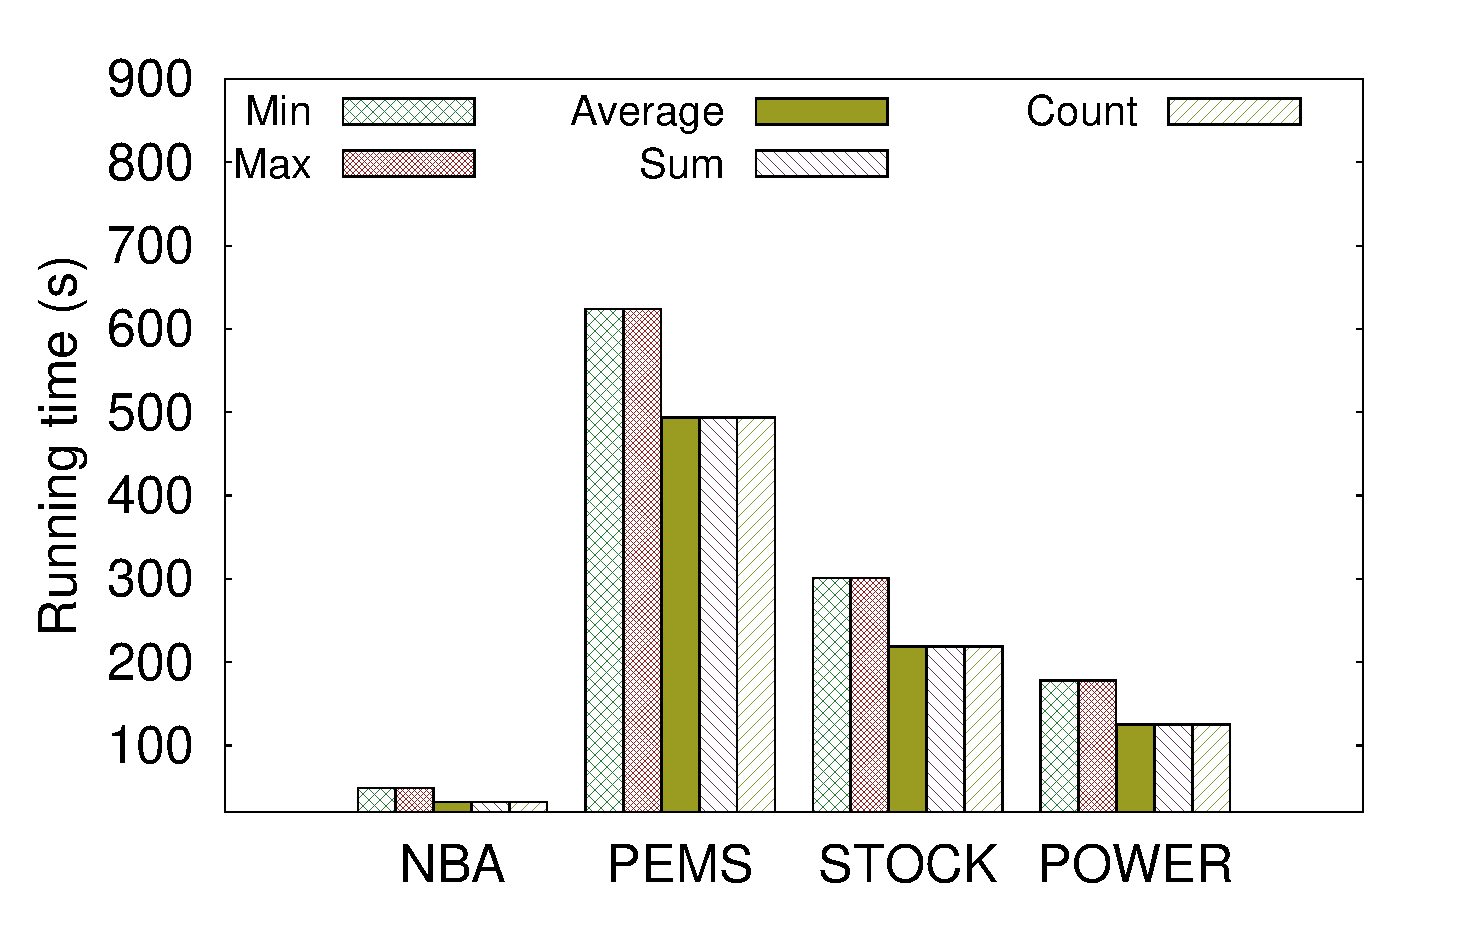
\includegraphics[width=\textwidth]{chapter4/exp/agg/agg_offline.eps}
        \vspace{-1.5em}
        \caption{Offline Scenario}
    \end{subfigure}
    \begin{subfigure}[b]{0.45\textwidth}
        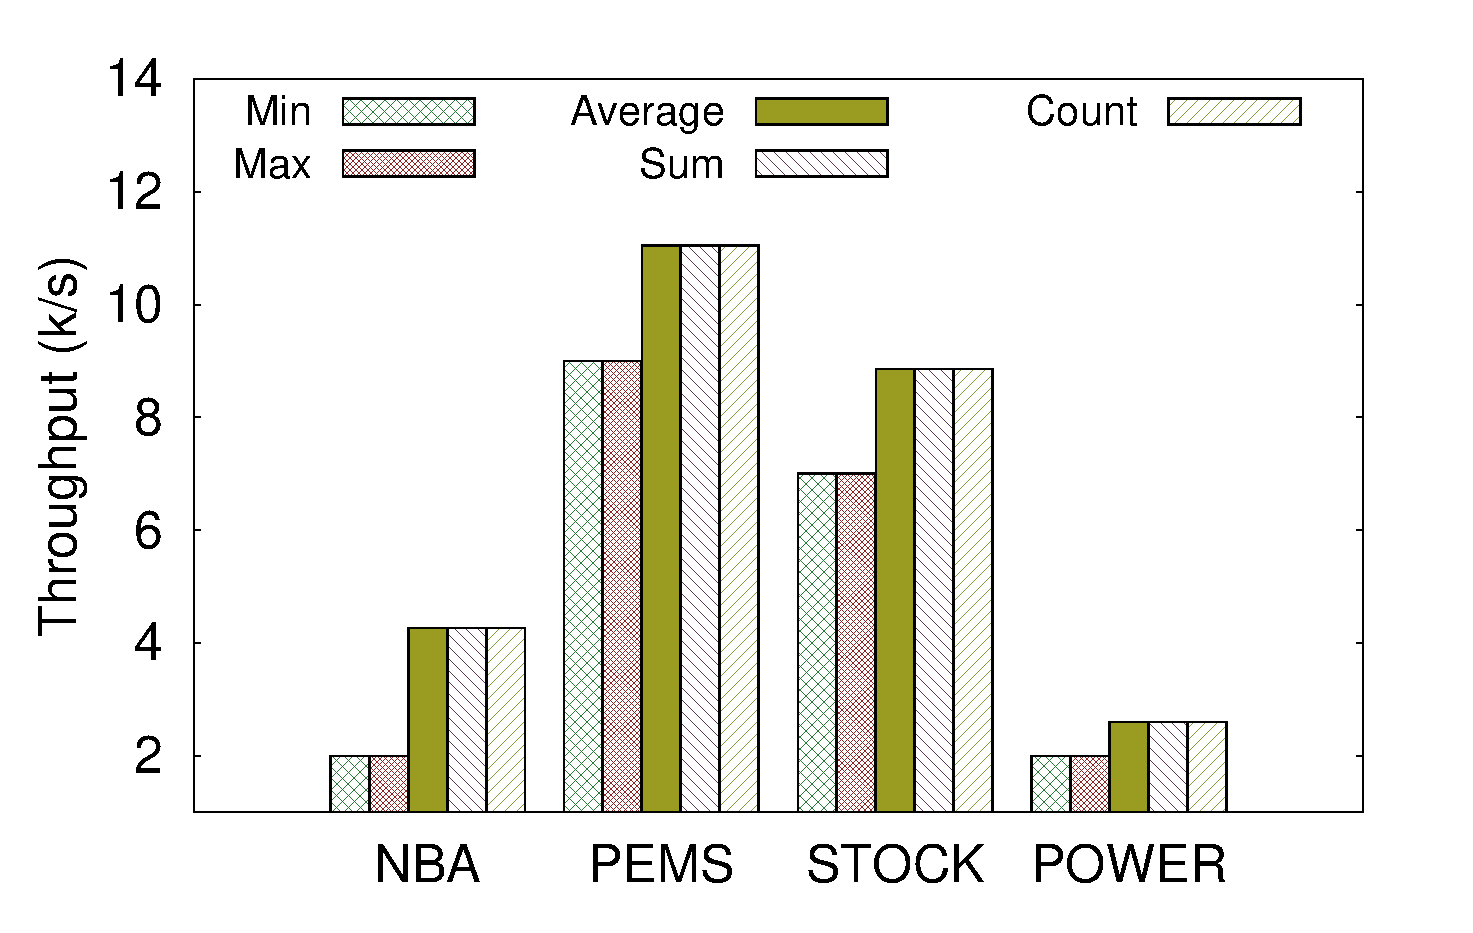
\includegraphics[width=\textwidth]{chapter4/exp/agg/agg_online.eps}
        \vspace{-1.5em}
        \caption{Online Scenario}
    \end{subfigure}
\caption{Performance under different aggregate functions} 
\label{exp:agg_cmp}
\end{figure}

%In fact, all distributive aggregation functions can leverage similar 
%technics to support efficient pruning. 


%\begin{itemize}
%\item \emph{sum}: $J_s(w) \leq J_s(w_1) + J_s(w-w_1) $
%\item \emph{min}: $J_s(w) \leq max(J_s(w_1), J_s(w-w_1))$
%\end{itemize}
%\noindent\textbf{Visting-Window Bound}
%\begin{itemize}
%\item \emph{sum}: $J_s(w) = J_s(w-1)+J_s(1)$
%\item \emph{min}: $J_s(w) = J_s(w/2)$
%\end{itemize} 
%\noindent\textbf{Unseen-Window Bound}
%\begin{itemize}
%\item \emph{sum}:$M_s(w) =\lfloor \mathbb{H}_s /w\rfloor J_s(w) + J_s(w-1)$
%\item \emph{min}: $M_s(w) = max\{J(w), J(1)\}$
%\end{itemize}
%\noindent\textbf{Online-Window Bound}
%\begin{itemize}
%\item \emph{sum}:$M_s(w) = W_s(t,w).\overline{v} + J_s(t-w)$
%\item \emph{min}:$M_s(w) = max\{W_s(t,w).\overline{v}, J(1)\}$
%\end{itemize}





\section{Proofs of Theorems in Chapter 5}
\subsection{Proofs of Theorem~\ref{THM:SPM_LB} and~\ref{THM:SPM_LB_INC}}
\label{apx:thm2proof}

\begin{proof}
$\Gamma$ can be formalized using linear algebra:
Let $G_A$ be an aggregated graph, with a $n \times n$ adjacent matrix $J$.
Since a vertex order is a permutation of $J$, the adjacent matrices 
of any reordered graphs can be represented as $PJP^T$
where $P \in \mathbb{P}$ is a $n\times n$ \emph{permutation matrix}~\footnote{an identity matrix with rows shuffled}.
In star partitioning, we assign each edge $e(i,j)$ in $G_A$ to the lower vertex, 
then the matrix $B=\triu(PJP^T)$~\footnote{\text{triu} is the upper triangle part of a matrix}
represents the assignment matrix wrt. $P$ (i.e., $b_{i,j} = 1$ if vertex $j$ is in star $Sr_i$).
Let vector $\vec{b}$ be the \textit{one}\footnote{every element in $\vec{b}$ is $1$} 
vector with size $n$. Let $\vec{c} = B\vec{b}$, then each $c_i$ 
denotes the number of edges in star $Sr_i$. Thus, $\Gamma$ can be represented
as the infinity norm of $B\vec{b}$. Let $\Gamma^*$ be the minimum $\Gamma$ among all vertex orderings, that is

\begin{equation}
\Gamma^* = \min_{P \in \mathbb{P}}{||B\vec{b}||_\infty} \text{ ,where } ||B\vec{b}||_\infty = \max_{1\leq j \leq n}(c_j)
\end{equation}

Let $B^*$ be the assignment matrix wrt. the optimal vertex ordering.
Since we have a star for each object, by the degree-sum formula and pigeon-hole theorem, 
$\Gamma^*=||B^*\vec{b}||_\infty \geq d/2$.
Next, for a vertex ordering $P$, let $e_{i,j}$ be an entry in $PAP^T$. Since 
edges in graph $G$ are independent, then $e_{i,j}$s are independent. 
Let $d_i$ denote the degree of vertex $i$, since a vertex ordering does not
affect the average degree,
then $E[d_i]=E[\Sigma_{1\leq j \leq n}e_{i,j}]=d$. Therefore, 
entries in $B$ can be written as :

\begin{equation*}
b_{i,j} = \begin{cases}
			e_{i,j}, i>j \\
			0, otherwise
		  \end{cases}  
\end{equation*}

There are two observations. First, since $e_{i,j}$s are independent,
$b_{i,j}$s are independent. Second, since $i>j$ and $e_{i,j}$s are independent. 
$E[b_{i,j}] = E[e_{i,j}]E[i>j]= E[e_{i,j}]/2$.
As $c_i$ is a sum of $n$ independent 0-1 variables ($b_{i.j}$s). By linearity 
of expectations,
we get: $E[c_i] = E[\Sigma_{1\leq j \leq n} b_{i,j}]=E[\Sigma_{1\leq j \leq n} e_{i,j}]/2 = d/2$.
 Let $\mu =E[c_i] = d/2$, 
$t = \sqrt{n\log n}$, by Hoeffding's Inequality, the following holds:

\begin{equation*}
\begin{split}
	Pr(c_i \geq \mu + t) &\leq \exp(\frac{-2t^2}{n}) = \exp(-2\log n) = n^{-2}
\end{split}
\end{equation*}

The first step holds since all $b_{i,j}$ are 0-1 variables. 
Next, the event $(\max_{1 \leq j \leq n}(c_j) \geq \mu + t)$ can be viewed as
$\cup_{c_i} (c_i \geq \mu + t )$, by Union Bound, the following holds:
\begin{equation*}
\begin{split}
	Pr(\Gamma \geq \mu + t) &=Pr(\max_{1\leq j \leq n}(c_j) \geq \mu + t)  \\
		& = Pr(\cup_{c_i} (c_i \geq \mu + t )) \\
		&\leq \Sigma_{1 \leq i \leq n} Pr(c_i \geq \mu + t) = n^{-1} = 1/n
\end{split}
\end{equation*}
Substitute back $t$ and $\mu$, we achieve the following concise form:
\begin{equation*}
	Pr(\Gamma \geq (d/2 + \sqrt{n\log n})) \leq 1/n
\end{equation*}
This indicates the probability of $(\Gamma-d/2)$ being no greater than $ O(\sqrt{n\log n})$ is $(1-1/n)$. 
Since $\Gamma^* \geq d/2$, it follows with probability greater than $(1-1/n)$, 
the $\Gamma - \Gamma^*$ is no greater than $O(\sqrt{n\log n})$.
When the aggregated graph is \emph{dense} (i.e., $d\geq \sqrt{12 \log n}$),
the Chernoff Bound can be used to derive a tighter bound of 
$O(\sqrt{\log n}) $ following the similar reasoning.
\end{proof}

\subsection{Proof of Theorem~\ref{THM:SPM_CORRECT}}
\label{apx:spm_correct}
\begin{proof}
For soundness, let $P$ be a pattern enumerated by SPARE. For any two objects $o_1, o_2 \in P.O$, the edge $e(o_1,o_2)$ is a superset of $P.T$. By the definition of star, $o_1$ $o_2$ belong to the same cluster at every timestamps in $P.T$. As $P.T$ is a valid sequence, by the definition of GCMP, $P$ is a true pattern.
For completeness, let $P$ be a true pattern. Let $s$ be the object with smallest ID in $P.O$. We prove that $P$ must be output by Algorithm~\ref{algo:apriori_mining} form $Sr_s$. 
First, based on the definition of star, every object in $P.O$ appears in $Sr_s$. Since $P.T$ is decomposable, then by Lemma 3 $\forall O' \subseteq O$, the time sequence of $O'$ would not be eliminated by any $\mathtt{sim}$ operations.  Next, we prove at every iteration \emph{level} $\leq |P.O|$, $P.O \subset O_u$, where $O_u$ is the forward closure. We prove by induction. When $level$ = 2, it obviously holds. If $P.O \subset O_u$ at \emph{level $i$}, then any subsets of $P.O$ with size $i$ are in the candidate set. In \emph{level} $i+1$, these subsets are able to grow to a bigger subset (in last iteration, they grow to $P.O$). This suggests that no subsets are removed by Lines~\ref{code:output1-start}-\ref{code:output2-end}. Then, $P.O \subset U_{i+1}$ holds. In summary, $P.O$ does not pruned by simplification, monotonicity and forward closure, therefore $P$ must be returned by SPARE.
\end{proof}